\documentclass[11pt,a4paper]{book}
\usepackage{color}
\usepackage{graphicx}
\usepackage{CJK}
\usepackage{rotating}


\begin{document}

\title{this is a title}
\author{pl}
\date{the date is today}
\maketitle
\tableofcontents

%\mainmatter

\begin{CJK}{UTF8}{gbsn}
  \chapter1{
    哈哈 \LaTeX
  }
\end{CJK}

\section{section 1}
\subsection{section 2.1}

\linespread{1.3}
\paragraph{first contents}


\begin{CJK}{UTF8}{gbsn}
  你好 \LaTeX
  
You can mix latin letters and chinese.
\end{CJK}



this is some text of content of ``this'' subsection.\\
this is another line of content.


\section{formulas}{
  \centering{B$^2$ = {\bf B} $\times$ B}
  \begin{center}
    A[3] is $\mathrm{A}_3$
  \end{center}
}


\section{left and right}{
  \raggedright{text on left}
  \begin{flushleft}
    another text on left
  \end{flushleft}
  \raggedleft{text on right}
  \begin{flushright}
    another text on right
  \end{flushright}
}

\chapter{verbatim}
\begin{verbatim}
some thing verbatim \\ /23454234$&%^&^(*^\z@%@#$%
\end{verbatim}

\section{colors}
\definecolor{tianyi_blue}{RGB}{102,204,255}
\begin{figure}[!h]
  \centering
  \begin{turn}{45}
    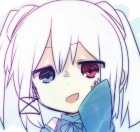
\includegraphics[width=0.5\textwidth,bb=0 0 140 132]{head_image.jpg}
  \end{turn}
  \caption{\color{tianyi_blue} title of image}
\end{figure}

\clearpage
\section{lists}
\begin{itemize}
\item item 1
\item item 2
\end{itemize}

\chapter{tables}
\section{common elements II}
\subsection{tabular}
this is a tabular: \\
\begin{tabular}{lcr||lcr}
  \hline
  \multicolumn{3}{|c|}{3$\times$3 matrix} \\
  \hline
  11 & 12 & 13 \\
  \hline
  21 & 22 & 23 \\
  \cline{1-2}
  31 & 32 & 33
\end{tabular}

\chapter{images}
\begin{figure}
  \begin{minipage}[b]{0.45\linewidth}
    \centering
    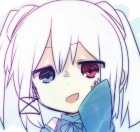
\includegraphics[natwidth=\linewidth,natheight=0.5\linewidth,scale=1]{head_image.jpg}
  \end{minipage}
  \begin{minipage}[b]{0.45\linewidth}
    \centering
    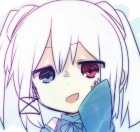
\includegraphics[natwidth=\linewidth,natheight=0.5\linewidth,scale=1]{head_image.jpg}
  \end{minipage}
  \label{fig:2img}
  \caption{2 images}
\end{figure}

\chapter{common errors -- part 4 of the lecture}{
  \section{notation and referance}{
    examples:  
\begin{verbatim}
\lable{marker}
...
\ref{marker}
...
\pageref{marker}
\end{verbatim}

we can ref the (figure:2img): \ref{fig:2img}
  }

  \section{more on figure}{
    on
\begin{verbatim}
\begin{figure}[!t]
\end{verbatim}
    
    the $[!t]$ notation means force the image shows on the top of the page. \\
    ps: \\
    $[!h]$ means put it here. \\
    $[!t]$ means put it on top. \\
    $[!b]$ means put it on bottom. \\
    $[!p]$ means put it into another page. \\
  }

  \section{footnote}{
    this is the footnote \footnote{the footnote text is here}
  }
  \section{hyper link}{
    use the package 'hyperref' \\
    $\backslash url\{http://the.url.is.here\}$ \\
    $\backslash href\{http://there.is.another.url\}$
    $\{$the link title or some discription$\}$
  }
  
  %\section{detial of formating images and tables}


  \section{errors and warings}{
    $\{\}$ miss match: Too many $\}$'s \\
    letter wrong like $\backslash dtae\{Mar.2014\}$: Undifined control sequence\\
    not in math mode: Not in Mathematics Mode. \\
    image or box are too large: Bad Boxes! \\
    missing packages: Missing Packages \\
  }
  
  \section{lengths}{
    normally don't override textlength setting or something like that.
  }
  \section{counters}{not normally used}
  \section{boxes}{
    add box on the text or something \\
    use $\backslash$framebox
  }
  \section{rules and struts}{
    make some area black or something like that
  }

}

\chapter{common errors -- part 5 of the lecture}{
  
}


\end{document}
